\documentclass{beamer}
\usepackage[utf8]{inputenc}
\usepackage{graphicx, epsfig}
\usepackage{amsmath,mathrsfs,amsfonts,amssymb}
\usepackage{floatflt}
\usepackage{epic,ecltree}
\usepackage{mathtext}
\usepackage{fancybox}
\usepackage{fancyhdr}
\usepackage{multirow}
\usepackage{enumerate}
\usepackage{epstopdf}
\usepackage{multicol}
\usepackage{algorithm}
\usepackage[noend]{algorithmic}
\usepackage{tikz}
\usepackage{blindtext}
\usetheme{default}%{Singapore}%{Warsaw}%{Warsaw}%{Darmstadt}
\usecolortheme{default}

\setbeamerfont{title}{size=\Huge}
\setbeamertemplate{footline}[page number]{}

\setbeamertemplate{section in toc}[sections numbered]


\makeatletter
\newcommand\HUGE{\@setfontsize\Huge{35}{40}}
\makeatother    

\setbeamerfont{title}{size=\HUGE}
\beamertemplatenavigationsymbolsempty

% latin bold lower
\newcommand{\ba}{\mathbf{a}} 
\newcommand{\bc}{\mathbf{c}} 
\newcommand{\be}{\mathbf{e}} 
\newcommand{\bh}{\mathbf{h}} 
\newcommand{\bp}{\mathbf{p}} 
\newcommand{\bt}{\mathbf{t}} 
\newcommand{\bs}{\mathbf{s}} 
\newcommand{\bu}{\mathbf{u}} 
\newcommand{\bv}{\mathbf{v}} 
\newcommand{\bw}{\mathbf{w}} 
\newcommand{\bx}{\mathbf{x}} 
\newcommand{\by}{\mathbf{y}} 
\newcommand{\bz}{\mathbf{z}} 

% latin bold upper
\newcommand{\bA}{\mathbf{A}} 
\newcommand{\bB}{\mathbf{B}} 
\newcommand{\bC}{\mathbf{C}} 
\newcommand{\bI}{\mathbf{I}} 
\newcommand{\bJ}{\mathbf{J}} 
\newcommand{\bL}{\mathbf{L}} 
\newcommand{\bM}{\mathbf{M}} 
\newcommand{\bP}{\mathbf{P}}
\newcommand{\bQ}{\mathbf{Q}} 
\newcommand{\bR}{\mathbf{R}} 
\newcommand{\bT}{\mathbf{T}} 
\newcommand{\bU}{\mathbf{U}} 
\newcommand{\bV}{\mathbf{V}} 
\newcommand{\bW}{\mathbf{W}} 
\newcommand{\bX}{\mathbf{X}} 
\newcommand{\bY}{\mathbf{Y}} 
\newcommand{\bZ}{\mathbf{Z}} 

% latin cal upper
\newcommand{\cF}{\mathcal{F}} 
\newcommand{\cG}{\mathcal{G}} 
\newcommand{\cI}{\mathcal{I}} 
\newcommand{\cL}{\mathcal{L}} 
\newcommand{\cM}{\mathcal{M}} 
\newcommand{\cN}{\mathcal{N}} 
\newcommand{\cS}{\mathcal{S}} 
\newcommand{\cT}{\mathcal{T}} 
\newcommand{\cW}{\mathcal{W}} 
\newcommand{\cX}{\mathcal{X}} 
\newcommand{\cZ}{\mathcal{Z}} 

% latin bb upper
\newcommand{\bbE}{\mathbb{E}} 
\newcommand{\bbI}{\mathbb{I}} 
\newcommand{\bbP}{\mathbb{P}} 
\newcommand{\bbR}{\mathbb{R}} 

% greek bold lower
\newcommand{\bepsilon}{\boldsymbol{\epsilon}} 
\newcommand{\btheta}{\boldsymbol{\theta}} 
\newcommand{\blambda}{\boldsymbol{\lambda}} 
\newcommand{\bpi}{\boldsymbol{\pi}} 
\newcommand{\bmu}{\boldsymbol{\mu}} 
\newcommand{\bsigma}{\boldsymbol{\sigma}} 
\newcommand{\bphi}{\boldsymbol{\phi}} 

% greek bold upper
\newcommand{\bSigma}{\boldsymbol{\Sigma}} 

\DeclareMathOperator*{\argmin}{arg\,min}
\DeclareMathOperator*{\argmax}{arg\,max}

\newcommand{\createdgmtitle}[1]{\title[\hbox to 56mm{Deep Generative Models  \hfill\insertframenumber\,/\,\inserttotalframenumber}]
	{\vspace{1cm} \\ Deep Generative Models \\ {\Huge Lecture #1}}
	\author{Roman Isachenko}
	\institute{
	Moscow Institute of Physics and Technology
	} 
	\date{2023, Autumn}
}

\usepackage{tikz}
\usetikzlibrary{arrows,shapes,positioning,shadows,trees}

\newcommand\myfootnote[1]{%
  \tikz[remember picture,overlay]
  \draw (current page.south west) +(1in + \oddsidemargin,0.5em)
  node[anchor=south west,inner sep=0pt]{\parbox{\textwidth}{%
      \rlap{\rule{10em}{0.4pt}}\raggedright\scriptsize \textit{#1}}};}

\newcommand\myfootnotewithlink[2]{%
  \tikz[remember picture,overlay]
  \draw (current page.south west) +(1in + \oddsidemargin,0.5em)
  node[anchor=south west,inner sep=0pt]{\parbox{\textwidth}{%
      \rlap{\rule{10em}{0.4pt}}\raggedright\scriptsize\href{#1}{\textit{#2}}}};}
      
\AtBeginSection[]
      {
      	\begin{frame}{Outline}
      		\tableofcontents[currentsection]
      	\end{frame}
      }
      \AtBeginSubsection[]{
      	\begin{frame}{Outline}
      		\tableofcontents[currentsection,currentsubsection]
      	\end{frame}
}
\createdgmtitle{13}

\usepackage{tikz}

\usetikzlibrary{arrows,shapes,positioning,shadows,trees}
%--------------------------------------------------------------------------------
\begin{document}
%--------------------------------------------------------------------------------
\begin{frame}[noframenumbering,plain]
%\thispagestyle{empty}
\titlepage
\end{frame}
%=======
\begin{frame}{Recap of previous lecture}
	\begin{block}{Forward gaussian diffusion process}
		\vspace{-0.4cm}
		\[
			\bx_t = \sqrt{1 - \beta} \cdot \bx_{t - 1} + \sqrt{\beta} \cdot \bepsilon, \quad \text{where }\bepsilon \sim \cN(0, 1);
		\]
		\[
			q(\bx_t | \bx_{t-1}) = \cN(\bx_t | \sqrt{1 - \beta} \cdot \bx_{t-1}, \beta \cdot \bI).
		\]
		\vspace{-0.7cm}
	\end{block}
	\begin{itemize}
		\item $p_{\infty}(\bx) = \cN(0, 1)$
		\item $q(\bx_t | \bx_0) = \cN(\bx_t | \sqrt{\bar{\alpha}_t} \cdot \bx_0, (1 - \bar{\alpha}_t) \cdot \bI)$
	\end{itemize}
	\begin{block}{Reverse gaussian diffusion process}
		\vspace{-0.2cm}
		\[
			p(\bx_{t - 1} | \bx_t, \btheta) = \cN \bigl(\bx_{t - 1} | \bmu(\bx_t, \btheta, t), \bsigma^2(\bx_t, \btheta, t)\bigr)
		\]
		\vspace{-0.5cm}
	\end{block}
	\begin{minipage}{0.5\linewidth}
		\begin{block}{Forward process}
			\begin{enumerate}
				\item $\bx_0 = \bx \sim \pi(\bx)$;
				\item $\bx_t = \sqrt{1 - \beta} \cdot \bx_{t - 1} + \sqrt{\beta} \cdot \bepsilon$, where $\bepsilon \sim \cN(0, 1)$, $t \geq 1$;
				\item $\bx_T \sim p_{\infty}(\bx) = \cN(0, 1)$.
			\end{enumerate}
		\end{block}
	\end{minipage}%
	\begin{minipage}{0.5\linewidth}
		\begin{block}{Reverse process}
			\begin{enumerate}
				\item $\bx_T \sim p_{\infty}(\bx) = \cN(0, 1)$;
				\item $\bx_{t - 1} = \bsigma(\bx_t, \btheta, t) \cdot \bepsilon + \bmu(\bx_t, \btheta, t)$;
				\item $\bx_0 = \bx \sim \pi(\bx)$;
			\end{enumerate}
		\end{block}
	\end{minipage}
	\myfootnotewithlink{https://lilianweng.github.io/posts/2021-07-11-diffusion-models/}{Weng L. What are Diffusion Models?, blog post, 2021}
\end{frame}
%=======
\begin{frame}{Recap of previous lecture}
	\vspace{-0.2cm}
	\begin{figure}
		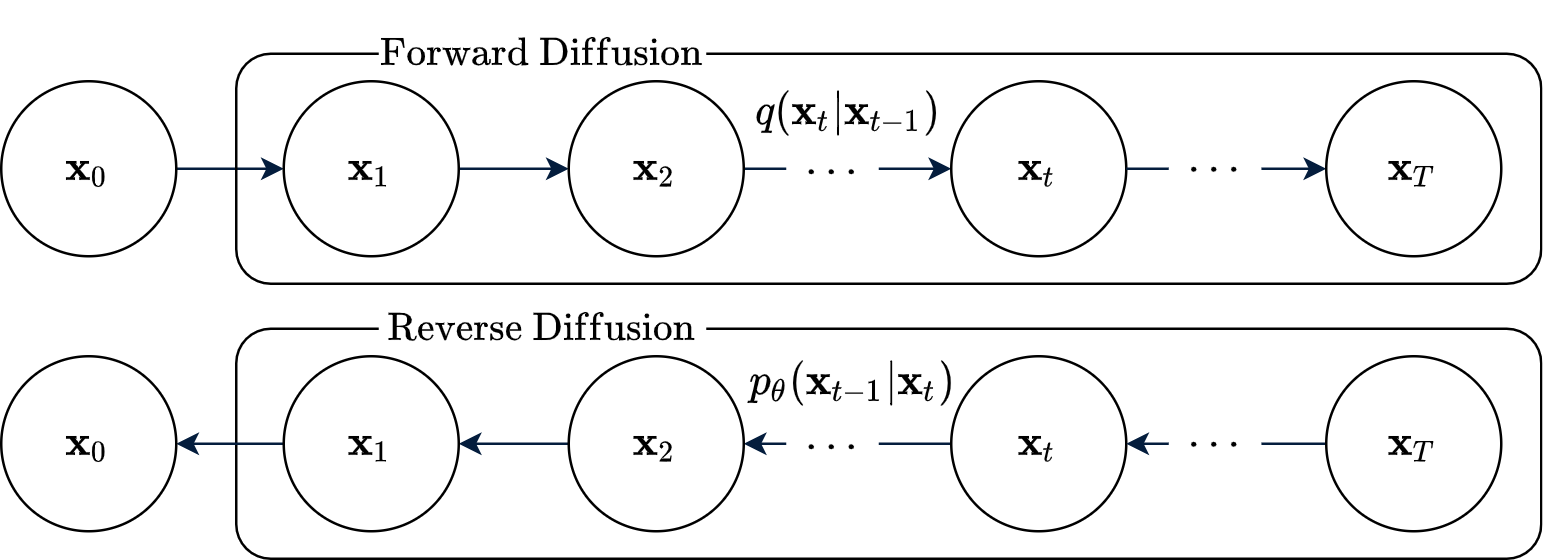
\includegraphics[width=0.65\linewidth]{figs/diffusion_pgm}
	\end{figure}
	\begin{itemize}
		\item Let treat $\bz = (\bx_1, \dots, \bx_T)$ as a latent variable (\textbf{note:} each $\bx_t$ has the same size).
		\item Variational posterior distribution (\textbf{note:} there is no learnable parameters)
		\vspace{-0.4cm}
		\[
			q(\bz | \bx) = q(\bx_1, \dots, \bx_T | \bx_0) = \prod_{t = 1}^T q(\bx_t | \bx_{t - 1}).
		\]
		\vspace{-0.5cm}
		\item Probabilistic model
		\vspace{-0.2cm}
		\[
			p(\bx, \bz | \btheta) = p(\bx | \bz, \btheta) p(\bz | \btheta)
		\]
		\item Generative distribution and prior
		\vspace{-0.3cm}
		\[
			p(\bx | \bz, \btheta) = p(\bx_0 | \bx_1, \btheta); \quad 
			p(\bz | \btheta) = \prod_{t=2}^T p(\bx_{t - 1} | \bx_t, \btheta) \cdot p(\bx_T)
		\]
	\end{itemize}
	\myfootnotewithlink{https://ayandas.me/blog-tut/2021/12/04/diffusion-prob-models.html}{Das A. An introduction to Diffusion Probabilistic Models, blog post, 2021}
\end{frame}
%=======
\begin{frame}{Outline}
	\tableofcontents
\end{frame}
%=======
\section{Overview of DDPM and link to score matching}
%=======
\begin{frame}{Denoising diffusion probabilistic model (DDPM)}
	\begin{block}{DDPM is a VAE model}
		\begin{itemize}
			\item Encoder is a fixed Gaussian Markov chain.
			\item Latent variable is a hierarchical (in each step the dim. of the latent equals to the dim of the input).
			\item Decoder is a simple Gaussian model.
			\item Prior distribution is given by parametric Gaussian Makov chain.
		\end{itemize}
	\end{block}
	\begin{minipage}{0.5\linewidth}
		\begin{block}{Forward process}
			\begin{enumerate}
				\item $\bx_0 = \bx \sim \pi(\bx)$;
				\item $\bx_t = \sqrt{1 - \beta} \cdot \bx_{t - 1} + \sqrt{\beta} \cdot \bepsilon$, where $\bepsilon \sim \cN(0, 1)$, $t \geq 1$;
				\item $\bx_T \sim p_{\infty}(\bx) = \cN(0, 1)$.
			\end{enumerate}
		\end{block}
	\end{minipage}%
	\begin{minipage}{0.5\linewidth}
		\begin{block}{Reverse process}
			\begin{enumerate}
				\item $\bx_T \sim p_{\infty}(\bx) = \cN(0, 1)$;
				\item $\bx_{t - 1} = \bsigma(\bx_t, \btheta, t) \cdot \bepsilon + \bmu(\bx_t, \btheta, t)$;
				\item $\bx_0 = \bx \sim \pi(\bx)$;
			\end{enumerate}
		\end{block}
	\end{minipage}
\end{frame}
%=======
\begin{frame}{Gaussian diffusion model vs Score matching}
	\vspace{-0.3cm}
	\[
		\cL_t = {\color{olive}\bbE_{\bepsilon}} \left[ \frac{\beta_t^2}{2\tilde{\beta}_t (1 - \beta_t)} \left\| {\color{violet}\frac{\bepsilon}{\sqrt{1 - \bar{\alpha}_t}}} - {\color{teal}\frac{\bepsilon(\bx_t, \btheta, t)}{\sqrt{1 - \bar{\alpha}_t}}}\right\|^2 \right]
	\]
	\begin{itemize}
		\item Result from Statement 2
		\[
			q(\bx_t | \bx_0) = \cN(\bx_t | \sqrt{\bar{\alpha}_t} \cdot \bx_0, (1 - \bar{\alpha}_t) \cdot \bI).
		\]
		\item Score of noised distribution
		\[
			\nabla_{\bx_t} \log q(\bx_t | \bx_0) = - \frac{\bepsilon}{\sqrt{1 - \bar{\alpha}_t}}, \quad \text{where } \bepsilon \sim \cN(0, 1).
		\]
		\item Let reparametrize our model: 
		\[
			\bs(\bx_t, \btheta, t) = - \frac{\bepsilon(\bx_t, \btheta, t)}{\sqrt{1 - \bar{\alpha}_t}}.
		\]
	\end{itemize}
	\begin{block}{Noise conditioned score network}
		\vspace{-0.2cm}
		\[
			{\color{olive}\bbE_{p(\bx' | \bx, \sigma_l)}}\bigl\| {\color{teal}\bs(\bx', \btheta, \sigma_l)} - {\color{violet}\nabla_{\bx'} \log p(\bx' | \bx, \sigma_l)} \bigr\|^2_2 \rightarrow \min_{\btheta}
		\]
	\end{block}
	\myfootnotewithlink{https://arxiv.org/abs/2006.11239}{Ho J. Denoising Diffusion Probabilistic Models, 2020}
	\end{frame}
%=======
\begin{frame}{Denoising diffusion probabilistic model (DDPM)}
	\begin{block}{Samples}
		\begin{figure}
			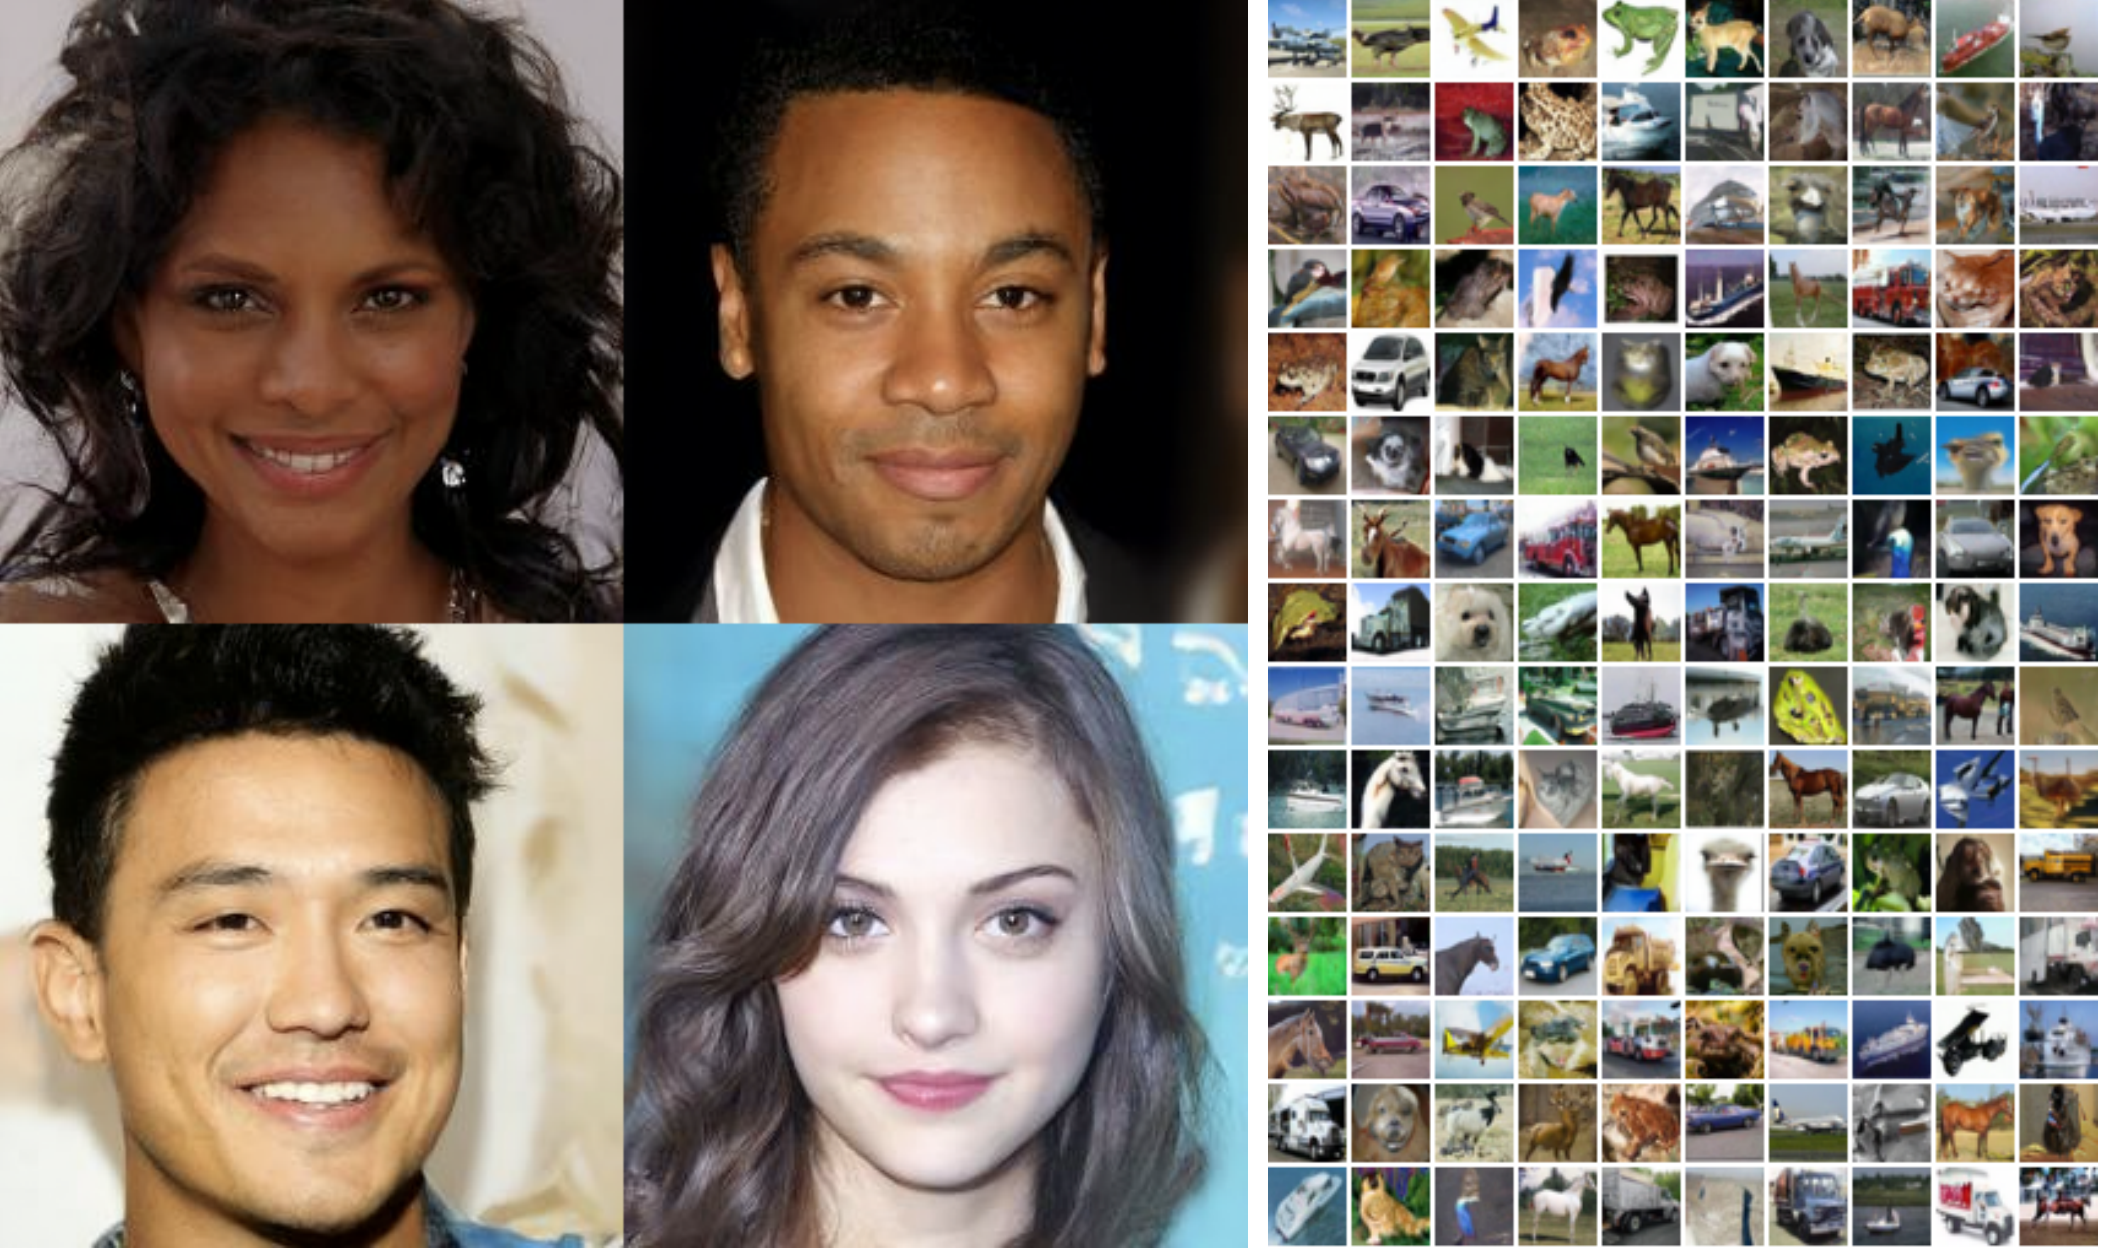
\includegraphics[width=\linewidth]{figs/ddpm_samples}
		\end{figure}
	\end{block}
	\myfootnotewithlink{https://arxiv.org/abs/2006.11239}{Ho J. Denoising Diffusion Probabilistic Models, 2020}
\end{frame}
%=======
\section{The worst course overview}
%=======
\begin{frame}{The worst course overview :)}
	\begin{figure}
		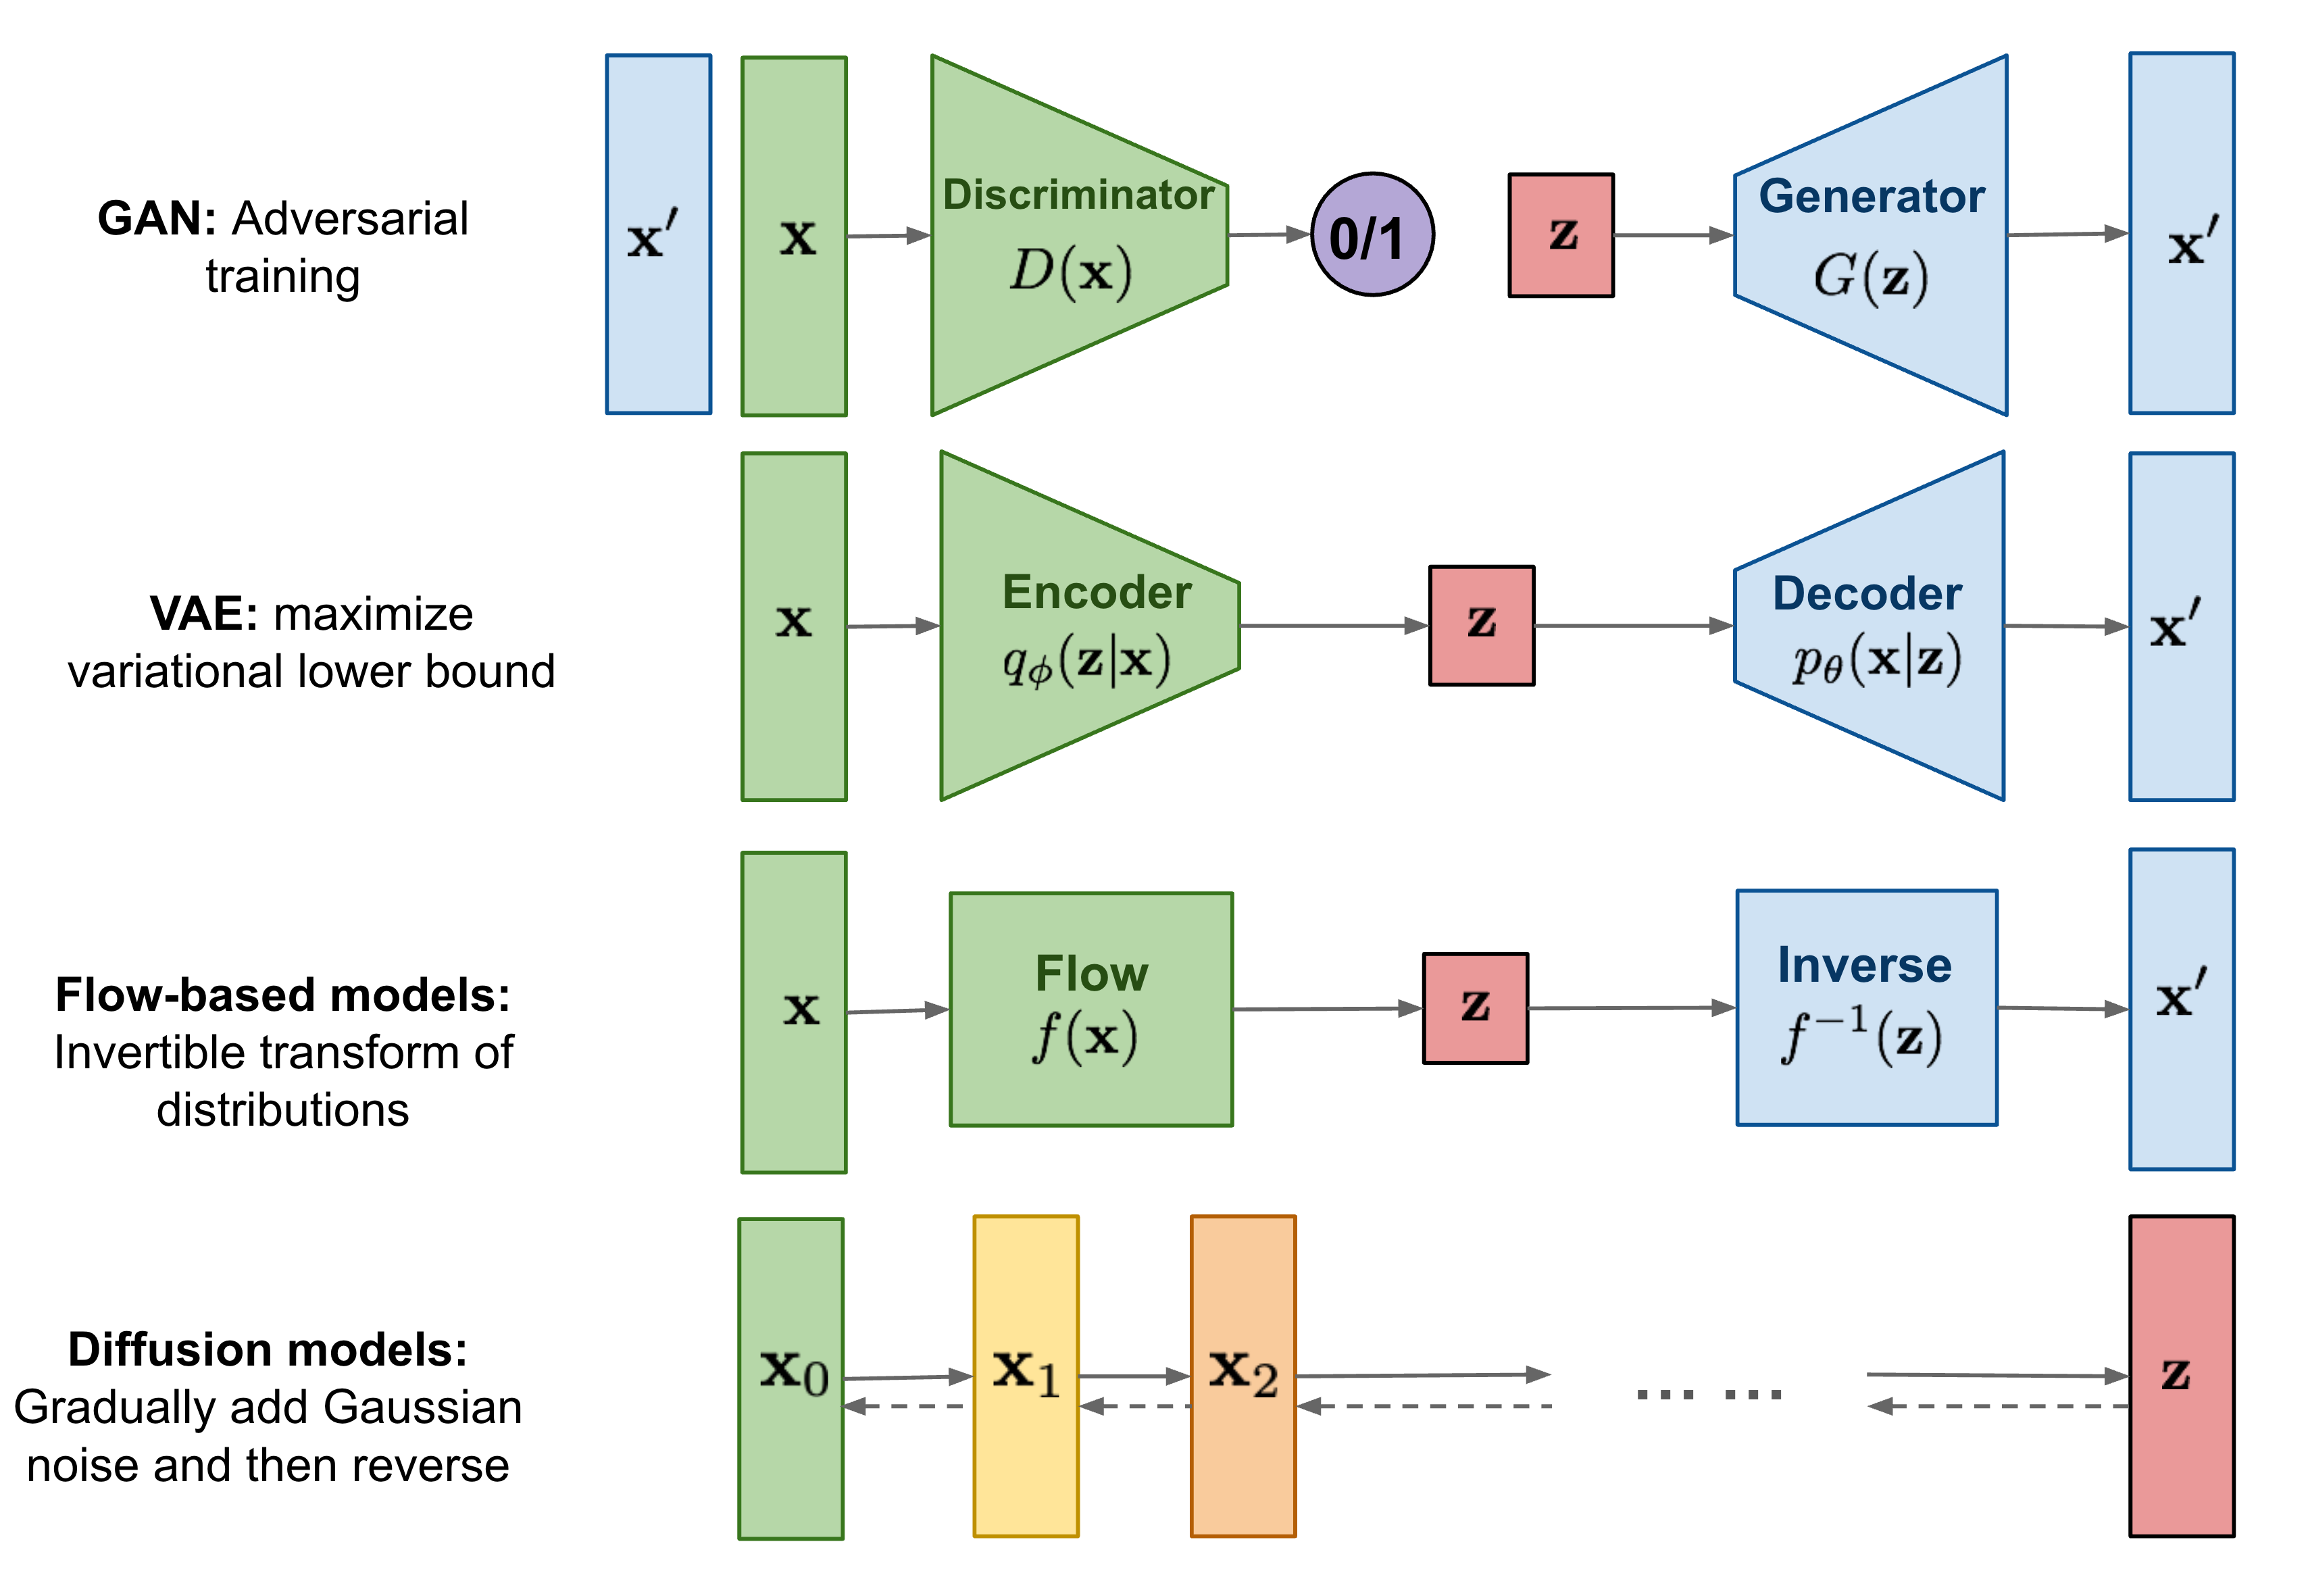
\includegraphics[width=\linewidth]{figs/generative-overview}
	\end{figure}
	\myfootnotewithlink{https://lilianweng.github.io/posts/2021-07-11-diffusion-models/}{Weng L. What are Diffusion Models?, blog post, 2021}
\end{frame}
%=======
\begin{frame}{The worst course overview :)}
	\begin{figure}
		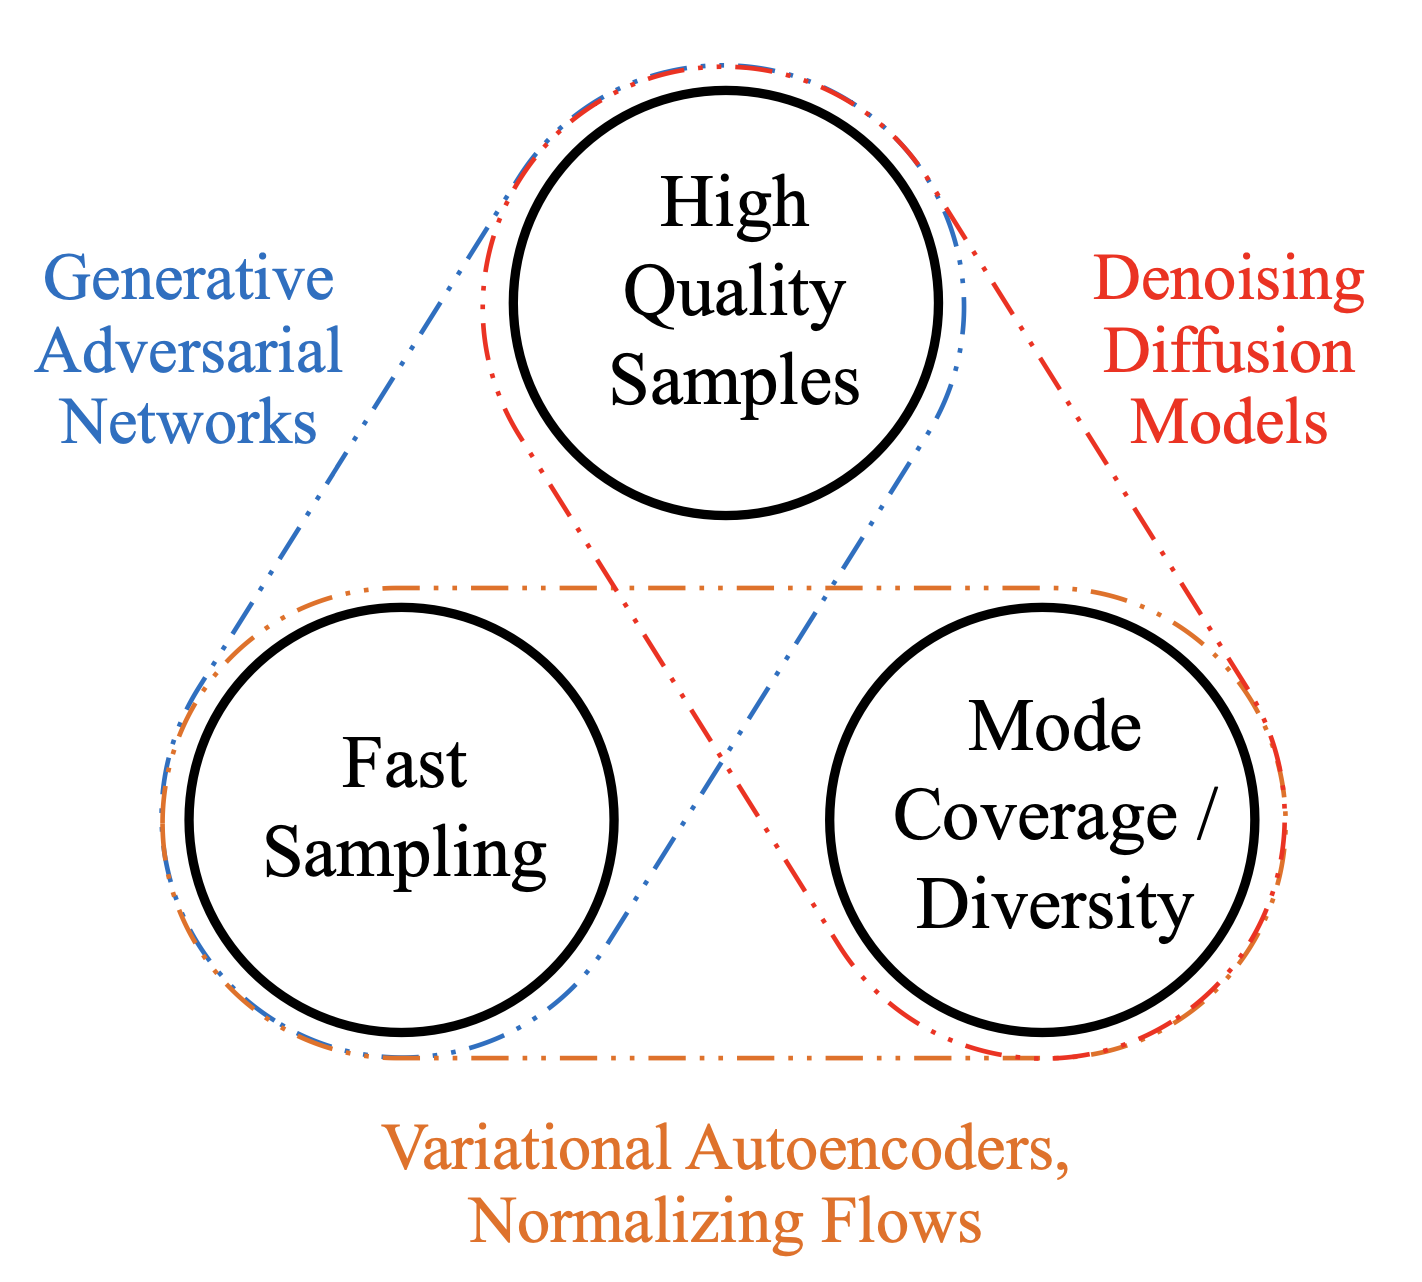
\includegraphics[width=0.7\linewidth]{figs/trilemma}
	\end{figure}
	\myfootnotewithlink{https://arxiv.org/abs/2112.07804}{Xiao Z., Kreis K., Vahdat A. Tackling the generative learning trilemma with denoising diffusion GANs, 2021}
\end{frame}
%=======
\begin{frame}{Summary}
	\begin{itemize}
		\item Objective of DDPM is closely related to the noise conditioned score network and score matching.
	\end{itemize}
\end{frame}
\end{document} 